\documentclass[12pt, a4paper]{article}

\usepackage{amsmath}
\usepackage{bm}
\usepackage{array}
\usepackage{amsmath}
\usepackage[portuguese]{babel}
\usepackage{chngpage}
\usepackage{float}
\usepackage[a4paper, margin=2cm]{geometry}
\usepackage{graphicx}
\usepackage{hyperref}
\usepackage{listings}
\usepackage{setspace}
\usepackage{xcolor}

\lstdefinestyle{codestyle}{
    commentstyle=\color{teal},
    keywordstyle=\color{blue},
    numberstyle=\ttfamily\color{gray},
    stringstyle=\color{red},
    basicstyle=\ttfamily\footnotesize,
    breakatwhitespace=false,
    breaklines=false,
    keepspaces=true,
    numbers=none,
    showspaces=false,
    showstringspaces=false,
    showtabs=false,
    tabsize=4
}
\lstset{style=codestyle}

\title{\Huge \textbf{Computação Gráfica \\ \Large Trabalho Prático -- Fase II}}
\date{30 de março 2025}
\author{Grupo 3}

\begin{document}

\begin{center}
    
\includegraphics[width=0.25\textwidth]{res/cover/EE-C.eps}
\end{center}

\chardef\_=`_
\onehalfspacing
\setlength{\parskip}{\baselineskip}
\setlength{\parindent}{0pt}
\def\arraystretch{1.5}

{\let\newpage\relax\maketitle}
\maketitle
\thispagestyle{empty}

\vspace*{\fill}

\begin{adjustwidth}{-2cm}{-2cm} % These values only need to be large enough to center the table
    \begin{center}
        \begin{tabular}{>{\centering}p{0.25\textwidth}
                        >{\centering}p{0.25\textwidth}
                        >{\centering}p{0.25\textwidth}
                        >{\centering\arraybackslash}p{0.25\textwidth}}
            
\includegraphics[width=3.5cm]{res/cover/A104437.png} &
            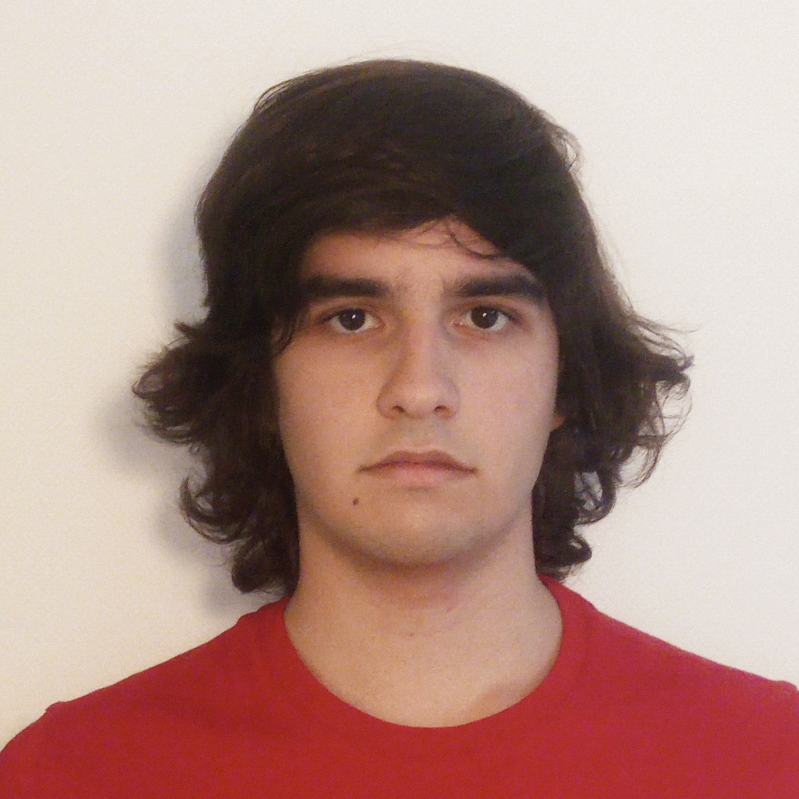
\includegraphics[width=3.5cm]{res/cover/A104348.png} &
            
\includegraphics[width=3.5cm]{res/cover/A90817.png} &
            
\includegraphics[width=3.5cm]{res/cover/A104179.png} \\

            Ana Oliveira & Humberto Gomes & Mariana Cristino & Sara Lopes \\
            A104437      & A104348        & A90817           & A104179
        \end{tabular}
    \end{center}
\end{adjustwidth}

\pagebreak

\begin{abstract}
    Para esta fase do trabalho prático, complementámos os programas \texttt{generator} e
    \texttt{engine} previamente desenvolvidos. Ao \texttt{generator}, adicionámos a possibilidade
    de gerar uma cena com o Sistema Solar, e modelos com rodas dentadas, fitas de Möbius, e garrafas
    de Klein. À \texttt{engine}, adicionámos transformações geométricas dos objetos, uma interface
    com o utilizador, movimentos da câmara (livre e orbital), e \emph{frustum culling} baseado em
    esferas. Na próxima fase, pretendemos desenvolver sobre os resultados aqui obtidos para
    adicionar diversas outras funcionalidades, explorando curvas de Bézier e de Catmull-Rom para a
    geração e animação de modelos, respetivamente.
\end{abstract}

\section{\emph{Generator}}

\subsection{Geração do Sistema Solar Estático}

O sistema solar foi representado por um uma estrutura hierárquica, definida de acordo com a atração
gravítica real dos corpos celestes. No topo da hierarquia, encontra-se o Sol, que serve de ponto
central e de referência para a órbita dos restantes corpos celestes. Cada planeta foi colocado num
grupo independente, filho do grupo do Sol. Quando aplicável, os satélites naturais (luas) e os anéis
dos planetas são inseridos como grupos filhos do planeta correspondente, preservando a hierarquia
entre os corpos. As cinturas de asteroides, por sua vez, são representadas como grupos filhos do
Sol, uma vez que orbitam em torno dele.

Cada grupo define as transformações aplicadas aos seus elementos, como translações, rotações, e
escalas, que são acumuladas ao longo da árvore de grupos, ou seja, as transformações são aplicadas
sequencialmente e as transformações de cada corpo são relativas ao seu elemento pai. Esta
organização simplifica a expressão das translações e escalas relativas dos corpos celestes. Ademais,
apesar de não haver movimento do sistema solar neste momento, esta estrutura hierárquica torna mais
fácil que, no futuro:

\begin{itemize}
    \item os planetas orbitem em torno do Sol;
    \item as luas orbitem em torno do planeta a que pertencem;
    \item os anéis acompanhem o seu planeta respetivo;
    \item os asteroides se posicionem nas suas cinturas em órbitas relativas ao Sol.
\end{itemize}

A estrutura XML da cena gerada segue a hierarquia descrita anteriormente. Abaixo, apresenta-se um
exemplo de cena, apenas com o Sol, a Terra e a Lua:

\lstset{language=xml}
\begin{lstlisting}

<group>
    <!-- Grupo do sol -->
    <group>
        <transform>
            <translate x="0"  y="0"  z="0" />
            <scale     x="30" y="30" z="30" />
        </transform>
        <models>
            <model file="../models/sphere.3d" />
        </models>
        <!-- Grupo da Terra -->
        <group>
            <transform>
                <translate x="28"  y="0"   z="-3" />
                <scale     x="0.2" y="0.2" z="0.2" />
            </transform>
            <models>
                <model file="../models/sphere.3d" />
            </models>
            <!-- Grupo da Lua -->
            <group>
                <transform>
                    <translate x="3"    y="0"    z="0" />
                    <scale     x="0.05" y="0.05" z="0.05" />
                </transform>
                <models>
                    <model file="../models/sphere.3d" />
                </models>
            </group>
        </group>
    </group>
</group>
\end{lstlisting}

Neste exemplo:
\begin{itemize}
    \item O grupo no topo da hierarquia contém o Sol, posicionado na origem e aumentado com
        uma escala (\texttt{scale}).
    \item Dentro do grupo do Sol, encontra-se a Terra, num grupo posicionado com uma translação
        (\texttt{translate}). O tamanho da Terra também é ajustado com uma escala.
    \item Dentro do grupo da Terra está a Lua, com a sua própria transformação relativa.
\end{itemize}

Além dos planetas e das luas, existem dois corpos celestes adicionais com formas de representação
específicas no XML:

\begin{itemize}
    \item As cinturas de asteroides são compostas por esferas, cubos e cilindros, escolhidos
        aleatoriamente. Estas figuras são adicionadas um a grupo filho do Sol, e são posicionadas
        com coordenadas aleatórias em torno de um raio definido. Cada asteroide recebe
        transformações próprias de translação, rotação e escala, simulando a dispersão e dimensão
        variável destes corpos celestes.

    \item Os anéis dos planetas utilizam o modelo de um \emph{torus}, gerado na primeira fase deste
        trabalho prático. Para simular a sua aparência achatada, é aplicada uma escala com fator
        inferior a $1$ no eixo $y$. Além disso, os anéis são orientados com uma rotação por um
        diferente eixo consoante o seu planeta.
\end{itemize}

Parte do sistema solar gerado pode ser observado na figura abaixo:

\begin{figure}[H]
    \centering
    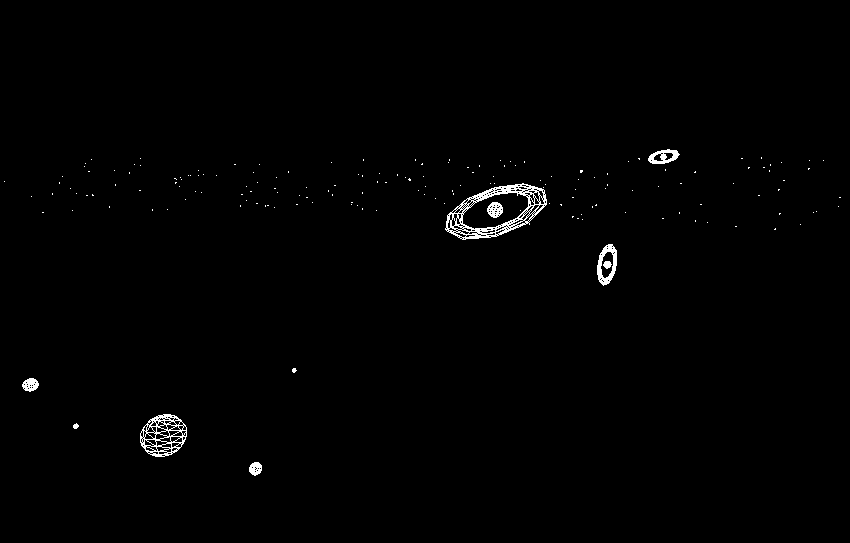
\includegraphics[width=0.9\linewidth]{res/phase2/results/SolarSystemOverview.png}
    \caption{Sistema solar com anéis e cinturas de asteroides visíveis.}
\end{figure}

O sistema solar pode ser gerado de forma personalizada, através dos seguintes parâmetros definidos
pelo utilizador, via linha de comando, especificados ao \texttt{generator} pela ordem apresentada
abaixo:

\begin{itemize}
    \item \texttt{sceneScale} -- Escala global, aplicada a toda a cena;
    \item \texttt{sunSizeFactor} -- Escala aplicada ao Sol;
    \item \texttt{planetSizeFactor} -- Escala aplicada aos planetas;
    \item \texttt{moonSizeFactor} -- Escala aplicada aos satélites naturais;
    \item \texttt{distanceFactor} -- Proporção da distância entre os diferentes corpos celestes;
    \item \texttt{asteroidBeltDensity} -- Densidade definida para as cinturas de asteroides;
    \item \texttt{ringSizeFactor} -- Proporção dos anéis em relação ao planeta.
\end{itemize}

Ainda existem muitas melhorias que podem ser feitas ao sistema solar, como o movimento dos corpos e
a adição de texturas, que se pretendem implementar ao longo das próximas fases do trabalho prático.

\subsection{Fita de Möbius}

Uma funcionalidade adicional que se implementou no \texttt{generator} foi a geração de fitas de
Möbius. Para gerar uma fita de Möbius, é necessário ter-se um raio, uma largura, o número de
\emph{slices}, o número de \emph{stacks}, e o ficheiro para onde será exportado o modelo gerado.
Ademais, uma fita de Möbius clássica possui uma torção (uma meia volta), mas para tornar a geração
da figura mais interessante, é possível variar de número de torções do modelo gerado. Abaixo,
apresenta-se a linha de comandos do \texttt{generator} que deve ser usada para gerar uma fita de
Möbius:

\texttt{./generator mobiusStrip <radius> <width> <twists> <slices> <stacks> <file>}

Matematicamente, as coordenadas de um ponto da \emph{fita de Möbius} são definidas do seguinte modo,
onde $R$, $W$ e $T$ são os parâmetros dados para a geração da \emph{fita de Möbius}, o raio, a
largura e o número de torções, respetivamente \cite{mobius-strip}:

\begin{minipage}{0.5\textwidth}
    $$
    x = \left (
            R + W \cdot \frac{\theta}{2} \cdot \cos \left ( T \cdot \frac{\phi}{2} \right )
        \right )
        \cdot \cos \phi
    $$
    $$
    y = W \cdot \frac{\theta}{2} \cdot \sin \left ( T \cdot \frac{\phi}{2} \right )
    $$
    $$
    z = \left (
            R + W \cdot \frac{\theta}{2} \cdot \cos \left ( T \cdot \frac{\phi}{2} \right )
        \right ) \cdot
        \sin \phi
    $$
\end{minipage}
\begin{minipage}{0.5\textwidth}
    $$\phi \in \left [ 0, 2 \pi \right [$$
    $$\theta \in \left [ -1, 1 \right ]$$
\end{minipage}

Para gerar uma nuvem de pontos uniformemente distribuídos, discretiza-se $\phi$ e $\theta$ em
\emph{slices} e \emph{stacks}, respetivamente, e percorre-se a faixa pelas suas fatias e camadas:

$$
\phi_i = i \cdot \frac{2\pi}{N_\text{slices}}
\hspace{1cm}
i \in \left \lbrace 0, 1, \ldots, N_\text{slices} \right \rbrace
$$

$$
\theta_j = j \cdot \frac{2}{N_\text{stacks}} -1
\hspace{1cm}
j \in \left \lbrace 0, 1, \ldots, N_\text{stacks} \right \rbrace
$$

Após a geração dos vértices, estes são agrupados nos triângulos que compõem a superfície da
fita de Möbius. Para isso, considera-se um vértice de referência, $P_1$, juntamente com o vértice
adjacente na mesma fatia, $P_3$, e os dois vértices correspondentes na fatia seguinte, $P_2$ e
$P_4$, como mostra a figura abaixo. Com estes quatro vértices, geram-se quatro faces triangulares:
duas faces voltadas para um lado e outras duas faces para o outro. Este processo repete-se para
todos os vértices onde é aplicável, garantindo que cada célula quadrangular é subdividida em
quatro triângulos, dois para cada lado.

\begin{figure}[H]
    \centering
    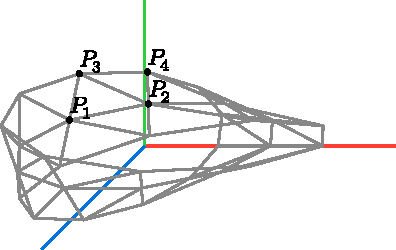
\includegraphics[width=0.45\textwidth]{res/phase2/figures/MobiusStrip.pdf}
    \caption{Pontos utilizados numa iteração da geração de faces da fita de Möbius.}
\end{figure}

Como a \emph{fita de Möbius} é uma superfície não orientável, deve ser possível ver os dois lados da
fita quando esta é desenhada. É por isto que se geram faces dos dois lados da fita: estes são
necessários para esta ser visualizada mesmo quando o \emph{back-face culling} está ativo. Para gerar
faces com diferentes orientações, a ordem em que os pontos são especificados é alterada conforme a
direção desejada. Por exemplo, para os quatro pontos apresentados acima, os triângulos gerados são
os seguintes:

$$
T_1 = (P_1, P_2, P_3)
\hspace{1cm}
T_2 = (P_2, P_1, P_3)
\hspace{1cm}
T_3 = (P_3, P_2, P_4)
\hspace{1cm}
T_4 = (P_2, P_3, P_4)
$$

\subsection{Garrafa de Klein}

Também foi implementada a geração outras superfícies não orientáveis, como a garrafa de Klein, que
não possui um lado interno e externo distinguíveis. A parametrização de um vértice sobre a garrafa
de Klein de raio $r$ pode ser definida pelas seguintes equações \cite{klein-bottle}:

$$
x = - \frac{2}{15} \; r \cos(\theta) \left (
        3  \cos \phi -
        30 \sin \theta +
        90 \cos^4 \theta  \sin \theta -
        60 \cos^6 \theta  \sin \theta +
        5  \cos \theta  \cos \phi  \sin \theta
    \right )
$$

\begin{align*}
    y = & - \frac{1}{15} \; r \sin(\theta) \left (
            3 \cos \phi -
            3 \cos^2 \theta  \cos \phi -
            48 \cos^4 \theta  \cos \phi +
            48 \cos^6 \theta  \cos \phi -
            60 \sin \theta
        \right .
    \\
    + & \left .
            5 \cos \theta  \cos \phi  \sin \theta -
            5 \cos^3 \theta  \cos \phi  \sin \theta -
            80 \cos^5 \theta  \cos \phi  \sin \theta +
            80 \cos^7 \theta  \cos \phi  \sin \theta
    \right)
\end{align*}

$$
z = \frac{2}{15} \; r (3 + 5 \cos \theta \sin \theta) \sin \phi
$$

A variável $\theta$ varia entre $0$ e $\pi$, e $\phi$ varia entre $0$ e $2\pi$. Para a geração dos
pontos da garrafa de Klein, os valores destas duas variáveis foram discretizados:

$$
\phi_i = i \cdot \frac{2\pi}{N_\text{slices}}
\hspace{1cm}
i \in \left \lbrace 0, 1, \ldots, N_\text{slices} \right \rbrace
$$
$$
\theta_j = j \cdot \frac{\pi}{N_\text{stacks}}
\hspace{1cm}
j \in \left \lbrace 0, 1, \ldots, N_\text{stacks} \right \rbrace
$$

Após a geração dos vértices, constroem-se as faces da garrafa de Klein. Cada quadrilátero entre duas
\emph{stacks} sucessivas é dividido em duas faces triangulares. Ao contrário da fita de Möbius,
decidiu-se que não era necessário renderizar o interior da garrafa, motivo pelo qual não se geram
quatro faces triangulares para cada quadrilátero.

\begin{figure}[H]
    \centering
    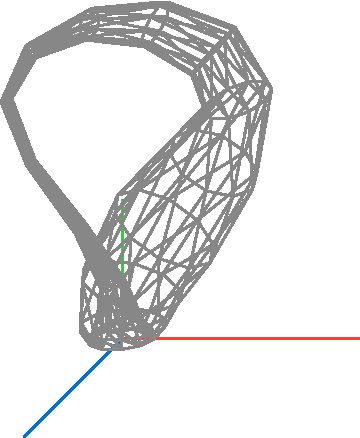
\includegraphics[width=0.35\textwidth]{res/phase2/figures/kleinBottle.pdf}
    \caption{Garrafa de Klein}
\end{figure}

Para usar o generator para gerar uma garrafa de Klein, a seguinte linha de comando deve ser
utilizada:

\begin{center}
    \texttt{./generator kleinBottle <radius> <slices> <stacks> <file>}
\end{center}

\subsection{Roda Dentada}

Também foi implementada a geração de rodas dentadas, que apresentam uma natureza muito semelhante à
de um cilindro: o seu interior é cilíndrico, e o seu exterior também o é, no entanto com variações
do raio nos dentes da roda dentada. A construção desta primitiva tem por base coordenadas
cilíndricas, onde a posição de cada ponto é definida em função do raio interno ($r_i$), do raio
externo ($r_e$), da altura do dente ($h_t$), do ângulo azimutal ($\phi$) e da altura da roda dentada
($h$).

A parametrização de um ponto sobre uma roda dentada pode ser definida pelas seguintes equações:

$$x = r \cos \phi$$
$$y \in \left [ 0, h \right ]$$
$$z =  r \sin \phi$$

No entanto, ao contrário do que acontece num cilindro, $r$ possui três valores distintos: para a
parte interna da roda, é utilizado $r_i$, para a parte externa, $r_e$, e nos dentes da roda,
$r_e + h_t$.

Para discretizar a superfície da roda dentada, divide-se o intervalo de $\phi$ em \emph{slices}, e
o intervalo de $y$ em \emph{stacks}. Assim, os incrementos destas variáveis são calculados da
seguinte forma:

$$
\Delta \phi = \frac{2\pi}{N_\text{slices}}
\hspace{1cm}
\Delta y = \frac{h}{N_\text{stacks}}
$$

É de notar que o número de fatias deve ser um múltiplo de 4 do número de dentes da roda dentada.
Caso contrário, irregularidades no modelo gerado podem ocorrer. Para evitar este problema, o número
de \emph{slices} é obrigatoriamente o $4 N_\text{dentes}$, que o utilizador especifica ao
\texttt{generator} juntamente com os outros parâmetros através da seguinte linha de comando:

\begin{adjustwidth}{-2cm}{-2cm} % These values only need to be large enough to center the text
    \begin{center}
        \texttt{
        ./generator gear <majorRadius> <minorRadius> <height> <stacks> <teeth> <toothHeight> <file>
        }
    \end{center}
\end{adjustwidth}

A construção dos vértices segue os seguintes passos:

\begin{itemize}
    \item Superfície lateral externa: Para cada \emph{stack}, os valores de $\phi$ são iterados,
        determinando a posição dos pontos ao longo da circunferência externa. Nos intervalos
        correspondentes aos dentes, o raio é aumentado em $h_t$, a altura do dente. passando a ser
        $r_e + h_t$.

    \item Superfície lateral interna: De forma similar à superfície lateral externa, é gerada a
        superfície interna do cilindro, mas o raio mantém-se constante em $r_i$.
\end{itemize}

Após a geração dos vértices, é necessário definir as faces triangulares que compõem a roda dentada.
A triangulação é realizada da seguinte forma:

\begin{itemize}
    \item Superfície lateral externa: Os pontos adjacentes de duas \emph{stacks} consecutivas são
        ligados, formando quadriláteros que são divididos individualmente em dois triângulos.

    \item Superfície lateral interna: É aplicada a mesma estratégia ao cilindro interno, com a
        ligação dos pontos entre diferentes \emph{stacks}.

    \item Bases superior e inferior: Os pontos da última \emph{stack} são ligados aos vértices
        centrais correspondentes, de modo a formar triângulos radiais.
\end{itemize}

\begin{figure}[H]
    \centering
    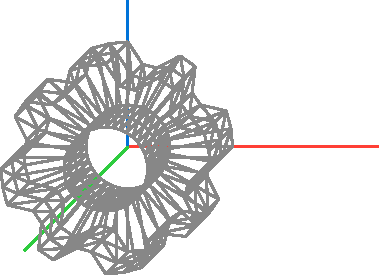
\includegraphics[width=0.45\textwidth]{res/phase2/figures/gear.pdf}
    \caption{
        \onehalfspacing
        Representação da estrutura da roda dentada. Note que a orientação dos eixos foi trocada para
        ser possível melhor observar os detalhes desta figura.
    }
\end{figure}

\section{\emph{Engine}}

\subsection{Transformações}

Um dos objetivos desta fase do trabalho prático é a possibilidade de aplicar transformações de
translação, rotação e escala às entidades na cena. Estas podem ser especificadas no ficheiro XML
como se apresenta no exemplo abaixo:

\lstset{language=xml}
\begin{lstlisting}

<group>
    <transform>
		<translate            x="1" y="2" z="3" />
        <rotate    angle="90" x="0" y="0" z="1" />
		<scale                x="1" y="2" z="1" />
    </transform>
    <models>
        <model file="modelo.3d" />
    </models>
</group>
\end{lstlisting}

Neste exemplo, a todos os modelos em \texttt{<models>} devem ser aplicadas, por esta ordem, uma
translação pelo vetor $(1, 2, 3)$, uma rotação de 90º pelo eixo $z$, e uma escala vertical por um
fator de duas vezes. Para calcular as matrizes associadas a cada uma destas transformações, as
funções \texttt{glm::translate}, \texttt{glm::rotate}, \texttt{glm::scale} são utilizadas.
\cite{glm-transform} Estas são semelhantes às funções \texttt{glTranslate}, \texttt{glRotate} e
\texttt{glScale} \cite{gl-transforms}, respetivamente, mas devolvem a matriz de transformação
calculada, em vez de modificarem as matrizes do estado interno do OpenGL. Outra diferença é que o
ângulo dado à função \texttt{glm::rotate} deve ser passado em radianos, sendo necessária uma
conversão do valor em graus presente na descrição XML da cena.

Para compor estas operações, as matrizes geradas pela \texttt{glm} são multiplicadas pela ordem em
que as transformações surgem no ficheiro XML. No exemplo anterior, onde $T$ é a matriz da
translação, $R$ a matriz de rotação, e $S$ a matriz de escala, as coordenadas no mundo dos pontos do
modelo devem ser multiplicadas pela matriz $W$ abaixo, originando as coordenadas no mundo do modelo
transformado:

$$
W = T R S
$$

Para desenhar as entidades no ecrã, é necessário também ter em conta a matriz da câmara, $C$, o
produto entre a matriz de projeção e a matriz de vista. Ademais, como os grupos na cena formam uma
hierarquia, é necessário considerar as transformações dos ascendentes de um grupo para o desenhar.
Assim, para desenhar a cena, usa-se uma \emph{stack} de matrizes, inicializada com a matriz da
câmara. Depois, para cada grupo aninhado, calcula-se o produto entre a matriz no topo do
\emph{stack} e a matriz de transformação do grupo, e esta matriz calculada é adicionada ao topo da
\emph{stack}. Quando se termina o desenho do grupo, é removida a matriz do topo da \emph{stack}. No
exemplo abaixo, mostra-se a \emph{stack} de matrizes durante o desenho de um grupo na hierarquia da
cena:

\begin{figure}[h]
    \begin{minipage}{0.5\textwidth}
        \centering
        \begin{tabular}{|>{\centering\arraybackslash}m{3cm}|}
            \hline \\
            \hline $C \cdot W_1 \cdot W_3 \cdot W_4$ \\
            \hline $C \cdot W_1 \cdot W_3$ \\
            \hline $C \cdot W_1$ \\
            \hline $C$ \\
            \hline
        \end{tabular}
    \end{minipage}
    \begin{minipage}{0.5\textwidth}
        \centering
        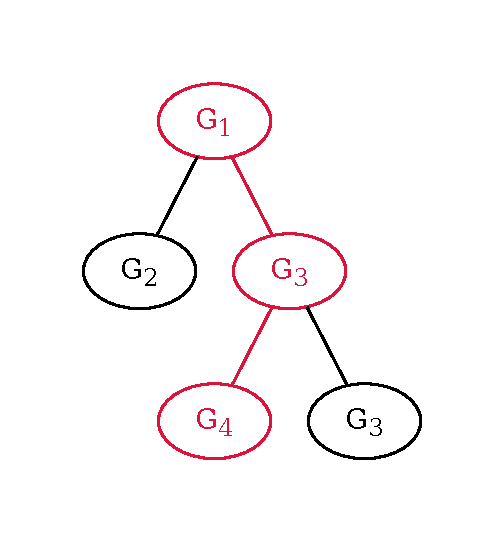
\includegraphics[width=0.6\textwidth]{res/phase2/SceneGraph.pdf}
    \end{minipage}
    \caption{\emph{Stack} de matrizes associada ao desenho de um grupo numa cena hierárquica.}
\end{figure}

\subsection{UI (Interface Gráfica)}

Como funcionalidade adicional, foi implementada uma interface gráfica, com o auxílio da biblioteca
\texttt{Dear ImGui}. \cite{dear-imgui} Esta biblioteca simplifica a gestão e atualização dos
componentes, pois os elementos gráficos são recriados a cada \textit{frame}.

A classe responsável pela configuração e renderização da interface é a \texttt{UI}. No processo de
inicialização realizado no seu construtor, a criação do contexto \texttt{ImGui} é realizada, bem
como a configuração do estilo da interface (o estilo \textit{Dark} foi escolhido por preferência dos
autores deste trabalho) e é efetuada a inicialização das implementações \texttt{OpenGL3} e
\texttt{GLFW} da biblioteca, algo que é necessário, visto que a biblioteca suporta diversos outros
\emph{backends}.

A interface é composta por um menu, sendo este renderizado na função \texttt{UI::render} com os
seguintes elementos:

\begin{itemize}
    \item Acompanhamento do Desempenho:
    \begin{itemize}
        \item FPS (\textit{Frames Per Second}): apresenta o número de \textit{frames}
            renderizados por segundo.
        \item Apresenta o número de entidades renderizadas em relação ao número total de entidades
            existentes. Esta métrica é útil para testar a eficiência do \textit{frustum culling},
            pois permite avaliar se apenas as entidades dentro da visão da câmara estão a ser
            renderizadas.
    \end{itemize}
    \item Configurações:
    \begin{itemize}
        \item Preenchimento de polígonos: permite alternar entre o preenchimento
            (\textit{fill polygons}) e o modo \textit{wireframe}.
        \item \textit{Back-face culling}: ativa ou desativa o \textit{back-face culling}.
        \item Exibir eixos: ativa ou desativa a visualização dos eixos.
        \item \textit{Bounding spheres}: ativa ou desativa a visualização das esferas encapsuladoras
            das entidades (ver \emph{frustum culling}).
    \end{itemize}
    \item Câmara: permite modificar as coordenadas da posição da câmara.
\end{itemize}

Após a definição dos elementos gráficos, a interface é renderizada através das funções
\texttt{ImGui::Render} e \texttt{ImGui\_ImplOpenGL3\_RenderDrawData}.

\begin{figure}[H]
    \centering
    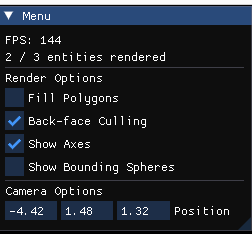
\includegraphics[width=0.35\textwidth]{res/phase2/UI.png}
    \caption{Interface Gráfica.}
\end{figure}

\subsection{Câmara Orbital}

A câmara orbital é uma câmara virtual que permite observar uma cena a partir de um ponto que orbita
à volta de ou de um objeto ou de um ponto fixo (\texttt{lookAt}). Na implementação atual, este ponto
de interesse está fixado na origem do espaço tridimensional. Esta abordagem é útil para observar um
objeto de diversos ângulos possíveis com o foco num ponto em específico.

A câmara orbital é definida por 3 parâmetros:

\begin{itemize}
    \item Raio ($r$): determina a distância do ponto de interesse à câmara;
    \item Ângulo azimutal ($\phi$): define a rotação da câmara em torno do eixo vertical,
    o que permite uma visualização de 360º em redor do objeto;
    \item Ângulo polar ($\theta$): controla o ângulo de elevação da câmara.
\end{itemize}

A atualização da posição da câmara é dada pela soma do ponto de interesse (\texttt{lookAt}) com
as coordenadas cartesianas obtidas a partir das coordenadas esféricas. As fórmulas utilizadas para
a conversão são as seguintes, tendo como ponto de interesse a origem do referencial:

$$x = r \sin \theta \cos \phi$$
$$y = r \cos \theta$$
$$z = r \sin \theta \sin \phi$$

De forma a garantir um comportamento estável e consistente, alguns valores devem ser restringidos a
intervalos pré-definidos. O raio encontra-se limitado entre $0.5$ e $100$, para evitar que a câmara
se aproxime demasiado ou se afaste demasiado do ponto de interesse. O ângulo azimutal varia entre
$0$ e $2\pi$, sendo reajustado quando a câmara completa uma volta. Impedir que este valor fique
demasiado alto ou demasiado baixo faz com que não sejam causados erros de precisão de vírgula
flutuante caso se deem milhões de voltas à câmara. Por fim, o ângulo polar encontra-se entre
$0.01$ e $\pi - 0.01$ para evitar que a câmara alcance os polos e cause instabilidade no
movimento. Sem esta restrição, caso $\theta > \pi$, o vetor $\vec{up}$ da câmara deixaria de ser
válido e a movimentação vertical da câmara ficaria invertida, tornando a navegação confusa e pouco
intuitiva.

Para controlar a câmara orbital, o utilizador utiliza o teclado, sendo que as teclas associadas a
cada ação são:

\begin{itemize}
    \item \texttt{W/S}: inclinar a câmara para cima e para baixo, respetivamente;
    \item \texttt{A/D}: rodar a câmara para a esquerda e para a direita, respetivamente;
    \item \texttt{F}: aproximar a câmara do ponto de interesse;
    \item \texttt{B}: afastar a câmara do ponto de interesse.
\end{itemize}

\subsection{Câmara Livre}

A câmara livre permite que o utilizador se desloque de forma intuitiva, sendo semelhante à de
jogos de exploração na primeira pessoa, como simuladores de voo, e ambientes de realidade
virtual.

A câmara pode deslocar-se e rodar de forma contínua no espaço tridimensional, sendo os seus
movimentos definidos pelos seguintes vetores:

\begin{itemize}
    \item Vetor $\vec{d}$: Direção do olhar da câmara.
    \item Vetor $\vec{r}$: Direção perpendicular ao vetor $\vec{d}$, ao longo do plano horizontal.
    \item Vetor $\vec{up}$: Aproximação do eixo vertical da câmara.
\end{itemize}

A posição da câmara, $P$, é atualizada de acordo com a seguinte equação:

$$
P' = P + v \cdot \vec{d'},
$$

onde $v$ representa a velocidade da câmara e $\vec{d'}$ a direção do movimento, que depende do
movimento escolhido pelo utilizador:

\begin{itemize}
    \item Translação horizontal: O movimento para a frente e para trás ocorre ao longo do vetor
        $\vec{d}$ ($\vec{d'} = \pm \widehat{d}$), enquanto o movimento lateral ocorre ao longo do
        vetor $\vec{r}$ ($\vec{d'} = \pm \widehat{r}$).
    \item Translação vertical: O movimento vertical acontece ao longo do vetor $\widehat{up}$
        ($\vec{d'} = \pm \widehat{up}$), permitindo ao utilizador subir e descer a câmara.
\end{itemize}

Para as transformações de rotação, é importante saber que a orientação da câmara é definida pelos
ângulos $\theta$ (\emph{yaw}), responsável pela rotação horizontal, e $\phi$ (\emph{pitch}),
responsável pela inclinação vertical. Ambos estes ângulos determinam a direção do vetor $\vec{d}$.
A atualização da orientação da câmara obtém-se através da conversão dos ângulos $\theta$ e $\phi$
para um vetor de direção tridimensional. A relação entre os ângulos e os componentes do vetor
$\vec{d}$ é dada por:

$$d_x = \cos \phi  \cos \theta$$
$$d_y = \sin \phi $$
$$d_z = \cos \phi  \sin \theta$$

Após serem calculados os componentes do vetor, este é normalizado, uma vez que é necessário
garantir que este mantém um comprimento unitário. Esta normalização é fundamental para garantir
que a câmara mantém uma velocidade constante em qualquer direção.

Além disso, foram tomadas medidas para prevenir o \emph{gimbal lock}. Este é um problema que ocorre
quando dois eixos de rotação se alinham, ou seja, quando $\phi$ atinge $90^\circ$ ou $-90^\circ$.
Além disso, no caso de $|\phi|$ exceder $90^\circ$, tal como na câmara livre, o \emph{vetor}
$\vec{up}$ deixa de ser válido e a movimentação vertical da câmara fica invertida. Para resolver
estes dois problemas, foi imposto o seguinte limite:

$$
-89^\circ \leq \phi \leq 89^\circ
$$

Este impede que a câmara olhe completamente para cima ou para baixo, garantindo que o vetor
$\vec{up}$ mantenha uma orientação bem definida e evitando a perda de controlo sobre a rotação
horizontal.

Sempre que a câmara sofre alterações, é necessário recalcular os seus vetores $\vec{r}$ e
$\vec{up}$. O vetor $\vec{r}$ é obtido como o produto externo entre a direção do olhar da câmara,
$\vec{d}$, e o vetor de referência vertical, $(0,1,0)$:

$$
\def\arraystretch{1}
\vec{r} = \vec{d} \times
\begin{bmatrix}
    0 \\ 1 \\ 0
\end{bmatrix}
$$

Depois, o vetor $\vec{up}$ é recalculado para ser ortogonal aos outros dois vetores:

$$
\vec{up} = \vec{r} \times \vec{d}
$$

Isto assegura que os movimentos laterais, verticais e de rotação permanecem coerentes em
qualquer orientação da câmara, garantindo um comportamento previsível para o utilizador. Ademais,
como a função \texttt{glm::lookAt} leva como argumento um ponto para o qual a câmara aponta, e
não o vetor $\vec{d}$, é necessário calcular as coordenadas de um ponto possível para gerar a nova
matriz de visualização:

$$
L = P + \vec{d}
$$

O utilizador pode controlar a câmara de forma intuitiva, utilizando o teclado para movimentação
e as setas direcionais para rotação:

\begin{itemize}
    \item \texttt{W/S}: Mover a câmara para a frente / trás, respetivamente;
    \item \texttt{A/D}: Mover a câmara para os lados esquerdo e direito, respetivamente;
    \item Espaço: Sobir a câmara;
    \item \emph{Shift} Esquerdo: Descer a câmara;
    \item Setas Esquerda / Direita: Rodar a câmara para a esquerda/direita;
    \item Setas Cima / Baixo: Inclinar a câmara para cima/baixo.
\end{itemize}

\subsection{\emph{Frustum Culling}}

Cada \emph{draw call} tem um custo elevado para o desempenho da aplicação. Logo, procurando reduzir
o número de \emph{draw calls}, foi implementado \emph{frustum culling}, para apenas ser requisitada
à GPU a renderização das entitidades totalmente ou parcialmente no \emph{view frustum} da câmara.

Seria muito computacionalmente intensivo verificar se a geometria de um modelo se encontra dentro ou
fora do \emph{view frustum}, pelo que se encapsulam todos os modelos em esferas que, devido à sua
geometria simples, permitem uma verificação rápida da sua visibilidade no \emph{view frustum}. No
entanto, visto que estas esferas podem ser um pouco maiores do que os modelos em si, é possível que
algumas entidades fora do ecrã sejam desenhadas, visto que parte das suas esferas ainda podem
intersetar os planos do \emph{view frustum}. Para mitigar este problema, formas geométricas
encapsuladoras mais complexas poderiam ser utilizadas, visto que estas se poderiam adaptar melhor à
geometria dos modelos. No entanto, o uso destas formas complexas conduziria a testes de visibilidade
mais caros, possivelmente anulando os benefícios de desenhar um menor número de entidades.

Quando um modelo é carregado, é necessário calcular a esfera que o encapsula. Em primeiro lugar, o
seu centro é calculado como o centro de massa de todos os pontos, como mostra a expressão abaixo,
onde $M$ é o modelo, uma sequência de pontos tridimensionais:

$$
C = \frac{1}{|M|} \sum_{p \in M} p
$$

Depois, o raio da esfera pode ser determinado como a distância entre o centro da esfera e o ponto
mais longínquo do mesmo, como mostra a expressão abaixo, onde $d$ é a função de distância cartesiana
entre dois pontos:

$$
r = \max \left \lbrace d(C, p) \mid p \in M \right \rbrace
$$

É também necessário saber como uma esfera encapsuladora é afetada quando o objeto que encapsula
sofre uma transformação no mundo. Considere-se uma matriz de transformação aplicada ao objeto (em
coordenadas do mundo), originada através da aplicação de translações, rotações, e escalas. A matriz
será 4x4 e terá o seguinte aspeto:

$$
\bgroup
    T =
    \begin{bmatrix}
        \vec \imath & \vec \jmath & \vec k & \vec t \\
        0 & 0 & 0 & 1
    \end{bmatrix}
\egroup
$$

Para calcular o centro da esfera após a transformação da entidade, basta multiplicar a matriz de
transformação pela posição do centro da esfera:

$$
C' = T C
$$

Depois, para calcular o novo raio da esfera, não é necessário ter em conta as transformações de
rotação, visto que as esferas são simétricas em todos os eixos possíveis. No entanto, é necessário
ter em conta a escala aplicada ao modelo. Por exemplo, na matriz $T$, a escala da entidade pelo
eixo $x$ é $\lVert \vec \imath \rVert$, e o mesmo se tem para o eixo $y$ e
$\lVert \vec \jmath \rVert$, e para $z$ e $\lVert \vec k \rVert$. Logo, o raio da esfera
transformada é:

$$
r' =
    \max
        \left ( \lVert \vec \imath \rVert, \lVert \vec \jmath \rVert, \lVert \vec k \rVert \right )
    \cdot
        r
$$

É possível tirar proveito da estrutura hierárquica da cena para otimizar o processo de
\emph{frustum culling}. Por exemplo, caso um grupo contenha várias entidades ou subgrupos, pode
construir-se uma esfera que encapsula a totalidade do grupo. Caso essa esfera não esteja no
\emph{view frustum}, pode-se evitar fazer os testes de visibilidade para as esferas dos objetos
individuais que compõem o grupo. Caso contrário, é na mesma necessário realizar esses testes.

O processo para determinar as características de uma esfera que encapsula todos os objetos de um
grupo é semelhante ao da construção de esferas com base no conjunto de pontos de um modelo. Em
primeiro lugar, para determinar o centro da esfera, calcula-se o centro de massa do conjunto de
pontos formado pelos centros de todas as esferas, $C$. De seguida, para cada subesfera, calcula-se
a sua distância máxima a $C$, o raio da subesfera adicionado à distância entre $C$ e o centro da
subesfera. Depois, a maior destas distâncias é escolhida para ser o raio da nova esfera, como mostra
a expressão abaixo, onde $S$ representa o conjunto de subesferas:

$$
r' = \max \left \lbrace d(C', C) + r \mid (C, r) \in S \right \rbrace
$$

Foi adicionada à \texttt{engine}, para depuração, a possibilidade de visualizar as esferas
encapsuladoras dos grupos e das entidades na cena. Abaixo, apresenta-se uma captura de ecrã da
\texttt{engine} com esta funcionalidade ativa:

\begin{figure}[H]
    \centering
    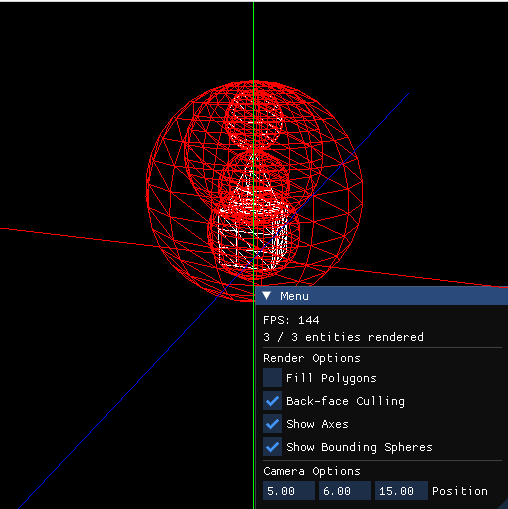
\includegraphics[width=0.4\textwidth]{res/phase2/BoundingSpheres.png}
    \caption{Esferas encapsuladoras de grupos e entidades.}
\end{figure}

Depois de saber como determinar as esferas encapsuladoras das entidades, é necessário determinar
o \emph{view fustum} da câmara, para se poder verificar a posição das esferas em relação aos planos
do \emph{view fustum}. Para determinar o \emph{view frustum}, é necessário obter alguns vetores
importantes da câmara \cite{lighthouse3d-frustum-planes}, os mesmos necessários para o funcionamento
da câmara livre, $\vec{d}$, $\vec{r}$ e $\vec{up}$. É importante também notar que o vetor $\vec{up}$
utilizado dado na descrição XML da cena pode não ser adequado para o cálculo do \emph{frustum}: é
necessário garantir que $\vec{up} \; \bot \; \vec{d}$. Para tal, o vetor $\vec{up}$ pode sofrer a
seguinte transformação:

$$
\vec{up} \leftarrow \left ( \vec{d} \times \vec{up} \right ) \times \vec{d}
$$

Além destes vetores, é também necessário conhecer as dimensões dos planos \emph{near} e \emph{far}.
Apesar de, matematicamente, planos não terem uma altura e uma largura, utiliza-se esta linguagem
para se referir às dimensões dos retângulos nestes planos que constituem o \emph{view frustum}. Na
expressão abaixo, mostra-se como se pode calcular a altura ($H_\text{near}$) e a largura
($W_\text{near}$) do plano \emph{near}. O processo para o plano \emph{far} é semelhante. Com o FOV
da câmara ($\theta$), a distância ao plano \emph{near} ($d_\text{near}$) e o \emph{aspect ratio}
(A), podem calcular-se as dimensões deste plano \cite{lighthouse3d-frustum-distances}:

$$
H_\text{near} = 2 d_\text{near} \tan \left ( \frac{\theta}{2} \right )
\hspace{1cm}
W_\text{near} = H_\text{near} A
$$

Com estes valores, é possível determinar as coordenadas dos pontos dos retângulos do
\emph{view frustum}. Os quatro pontos do plano \emph{near} (a amarelo na figura abaixo) podem ser
calculados do seguinte modo, e o método utilizado para o plano \emph{far} é semelhante
\cite{lighthouse3d-frustum-planes}:

$$
F = P +
    d_\text{near} \; \widehat{d} \; \pm
    \frac{H_\text{near}}{2} \; \widehat{up} \; \pm
    \frac{W_\text{near}}{2} \; \widehat{r} \;
$$

\begin{figure}[H]
    \centering
    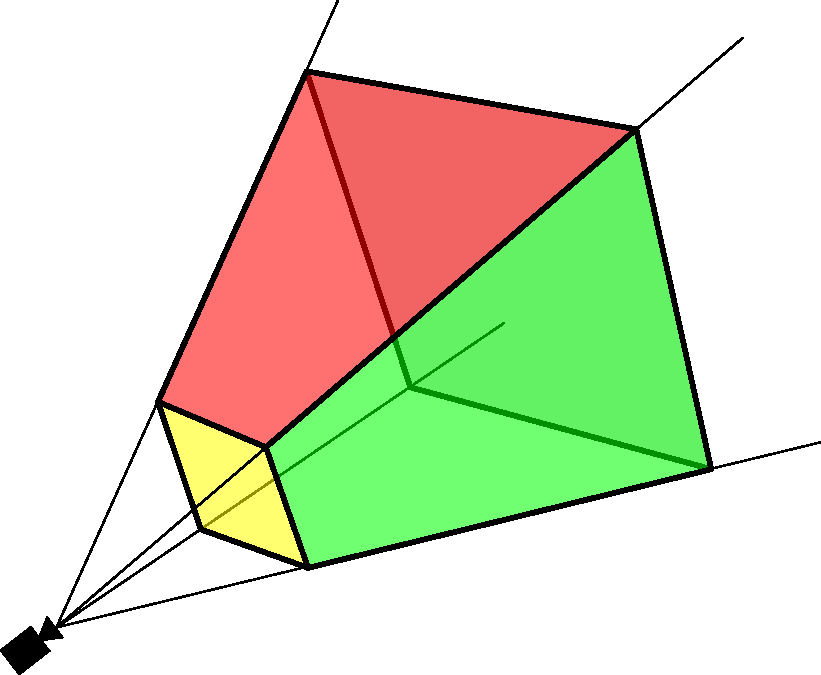
\includegraphics[width=0.4\textwidth]{res/phase2/ViewFrustum.pdf}
    \caption{\emph{View Frustum}.}
\end{figure}

Com os oito pontos do \emph{view frustum}, é possível determinar as equações cartesianas de cada
um dos seus planos, considerando três pontos da sua superfície. Em primeiro lugar, determina-se o
vetor normal ao plano. Com os três pontos, $P_1$, $P_2$ e $P_3$, determinam-se dois vetores, a
partir dos quais se calcula um produto externo, determinando-se assim um vetor perpendicular ao
plano \cite{lighthouse3d-plane}:

$$
n = \overrightarrow{P_1 P_2} \times \overrightarrow{P_1 P_3}
$$

Depois, com este vetor normalizado, é possível determinar a constante na equação cartesiana do plano
com base nas coordenadas de um dos três pontos dados \cite{lighthouse3d-plane}:

\begin{align*}
                       & \alpha x + \beta y + \gamma z + \delta = 0 \\
    \Leftrightarrow \; & \widehat{n} \cdot P + \delta = 0 \\
    \Leftrightarrow \; & \delta = -\widehat{n} \cdot P
\end{align*}

Durante a renderização de cada \emph{frame}, verificam-se que esferas estão totalmente ou
parcialmente dentro do \emph{view frustum}. Para uma esfera estar no \emph{view frustum} $F$, é
necessário que a distância assinada entre o centro da esfera e cada um dos planos do
\emph{view frustum} não seja inferior ao simétrico do seu raio, ou seja \cite{lighthouse3d-sphere}:

$$
\forall_{p \in F} \left ( \widehat{n} \cdot C + \delta \ge - r \right )
$$

Uma vez que é necessário calcular distâncias assinadas, é imperativo que os vetores normais de todos
os planos do \emph{view frustum} apontem para o seu interior, para que o conteúdo no seu interior (e
não no seu exterior) seja desenhado. \cite{lighthouse3d-frustum-planes} Por este motivo, a ordem em
que os pontos $P_1$, $P_2$ e $P_3$ são especificados é relevante.

\section{Resultados Obtidos}

Nesta secção, procuram-se apresentar algumas capturas de ecrã da \texttt{engine} das novas cenas
criadas e das cenas fornecidas pela docência da UC.

\subsection{Figuras Geométricas Geradas}

Os seguintes modelos foram criados utilizando o \texttt{generator}:

\begin{figure}[H]
    \centering
    \begin{minipage}{0.32\textwidth}
        \centering
        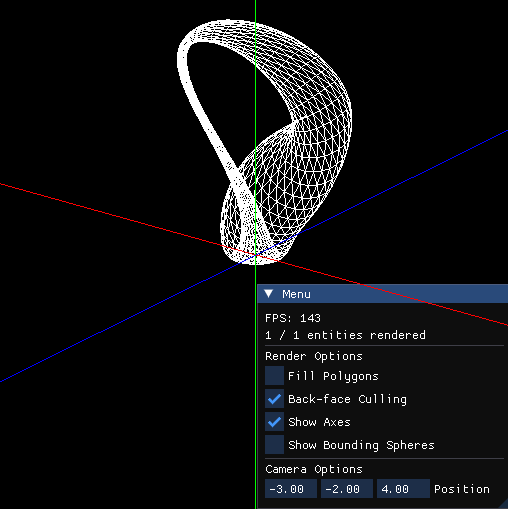
\includegraphics[width=0.8\textwidth]{res/phase2/results/KleinBottle.png}
        \caption{Garrafa de Klein.}
    \end{minipage}
    \begin{minipage}{0.32\textwidth}
        \centering
        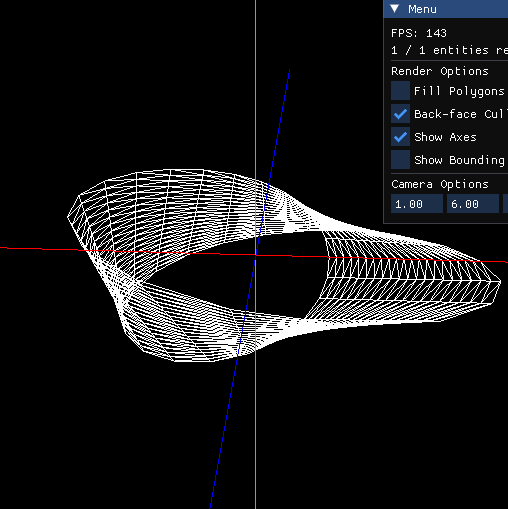
\includegraphics[width=0.8\textwidth]{res/phase2/results/MobiusStrip.png}
        \caption{Fita de Möbius.}
    \end{minipage}
    \begin{minipage}{0.32\textwidth}
        \centering
        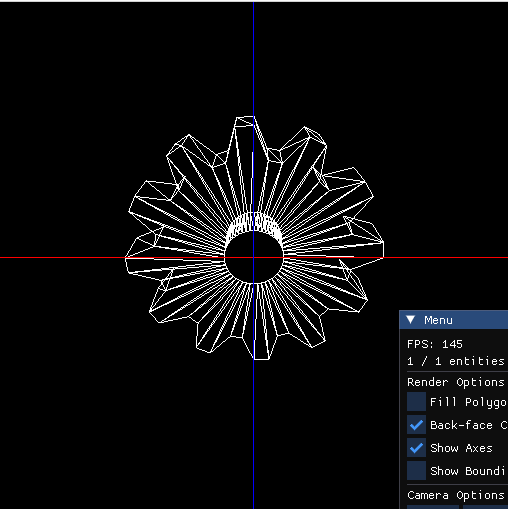
\includegraphics[width=0.8\textwidth]{res/phase2/results/Gear.png}
        \caption{Roda dentada.}
    \end{minipage}\hfill
\end{figure}

\subsection{Cenas fornecidas pela docência da UC}

A docência da UC forneceu, juntamente com o enunciado do trabalho, algumas cenas a serem testadas no
trabalho. A \texttt{engine} renderizou-as como esperado:

\begin{figure}[H]
    \begin{adjustwidth}{-2cm}{-2cm}
        \centering
        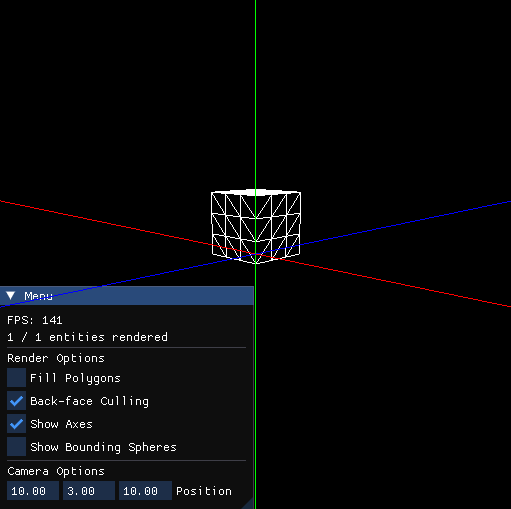
\includegraphics[width=0.26\textwidth]{res/phase2/results/Test1.png}
        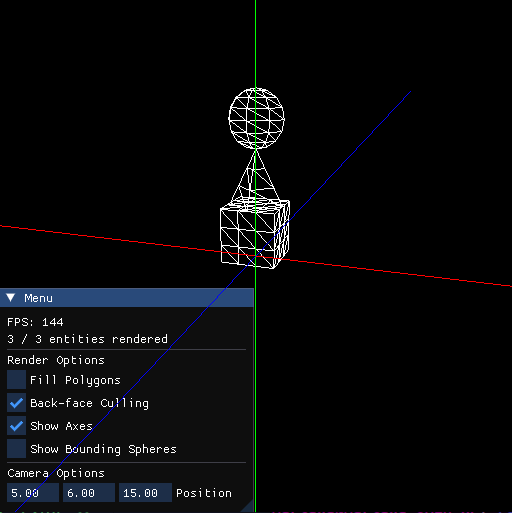
\includegraphics[width=0.26\textwidth]{res/phase2/results/Test2.png}
        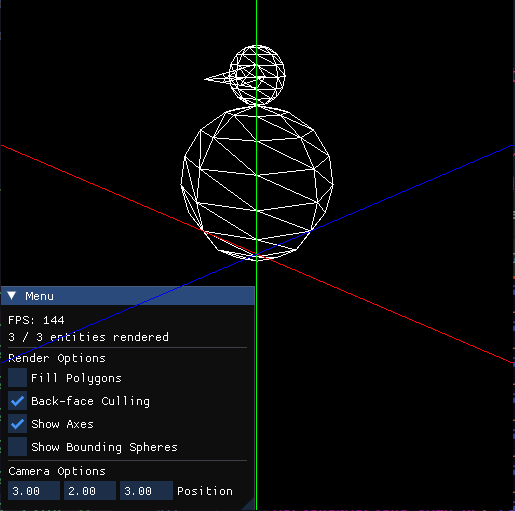
\includegraphics[width=0.26\textwidth]{res/phase2/results/Test3.png}
        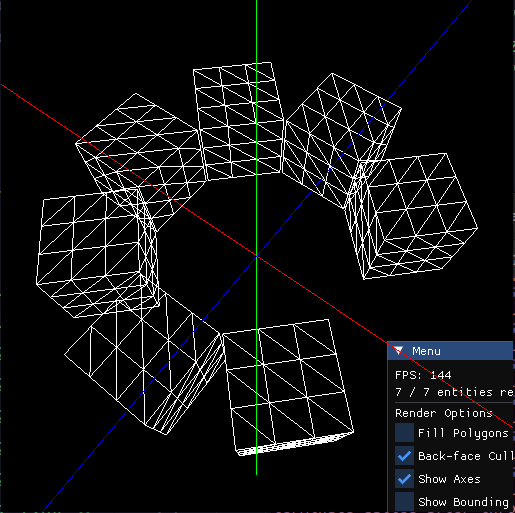
\includegraphics[width=0.26\textwidth]{res/phase2/results/Test4.png}
        \caption{Renderização das cenas de teste fornecidas pela docência da UC.}
    \end{adjustwidth}
\end{figure}

\section{Conclusão e Trabalho Futuro}

Consideramos que esta segunda fase deste trabalho prático foi concluída com sucesso. Em primeiro
lugar, não tivemos qualquer problema com a implementação das funcionalidades obrigatórias: as
transformações dos objetos nas cenas e a geração do Sistema Solar. Em relação aos objetivos que
tínhamos traçado na conclusão da última fase, conseguimos representar cenas numa estrutura
hierárquica, e implementar dois novos tipos de câmara, a câmara orbital e a câmara livre. No
entanto, não nos focámos na implementação da câmara em terceira pessoa, preferindo investir o nosso
tempo em outras funcionalidades que nos despertaram mais curiosidade. Todavia, ainda pretendemos
implementar este tipo de câmara, mas isso será algo para as próximas fases deste trabalho.

Além do que tínhamos planeado, implementámos diversas outras funcionalidades. Em primeiro lugar, do
lado do \texttt{generator}, implementámos diversas novas figuras, a roda dentada e alguns objetos
conhecidos da topologia, a fita de Möbius e a garrafa de Klein. Ademais, do lado da
\texttt{engine}, implementámos uma interface gráfica, para ser possível controlar vários parâmetros
possíveis da \texttt{engine}. Por último, implementámos também \emph{frustum culling}, para melhorar
o desempenho da \texttt{engine} através da redução do número de \emph{draw calls}.

Ao longo desta fase, a nossa principal dificuldade foi a implementação do \emph{frustum culling}.
Qualquer pequena falha (um sinal errado, uma troca entre duas variáveis, \emph{etc.}) pode fazer
com que este não funcione, pelo que foi necessário o desenvolvimento de uma boa infraestrutura
para depuração (como a apresentação das \emph{bounding spheres}) para encontrar e corrigir os erros
que fomos cometendo durante a implementação desta funcionalidade.

Para a próxima fase deste trabalho, desejamos implementar as funcionalidades obrigatórias pedidas,
a geração de modelos com base em \emph{patches} de Bézier, e a animação dos objetos da cena com
translações e rotações que variam ao longo do tempo. Além disso, como funcionalidades adicionais,
desejamos implementar a já mencionada câmara em terceira pessoa, bem como \emph{object picking} e
\emph{instanced rendering}.

\begingroup
\section{Bibliografia}
\renewcommand{\section}[2]{}

\begin{thebibliography}{9}
    \bibitem{mobius-strip}
        ``Möbius Strip.'' Wolfram MathWorld. Accessed: Mar. 25, 2025. [Online.] Available:
        \url{https://mathworld.wolfram.com/MoebiusStrip.html}
    \bibitem{klein-bottle}
        A. Norman and G. Newcomb, ``Klein surfaces and real algebraic function fields.'',
        \emph{Bulletin of the American Mathematical Society}, vol. 75, no. 4, pp. 869-872,
        Apr. 1969, \url{doi:10.1090/S0002-9904-1969-12332-3}.
    \bibitem{glm-transform}
        ``GLM\textunderscore EXT\textunderscore matrix\textunderscore transform''. GLM 0.9.9 API
        documentation. Accessed: Mar. 27, 2025. [Online.] Available:
        \url{https://glm.g-truc.net/0.9.9/api/a00247.html}
    \bibitem{gl-transforms}
        ``OpenGL (R) 2.1, GLX, and GLU Reference Pages ''. Khronos Registry.
        Accessed: Mar. 27, 2025. [Online.] Available:
        \url{https://registry.khronos.org/OpenGL-Refpages/gl2.1}
    \bibitem{dear-imgui}
        ``Dear ImGui.'' GitHub. Accessed: Mar. 2, 2025. [Online.] Available:
        \url{https://github.com/ocornut/imgui}
    \bibitem{lighthouse3d-frustum-planes}
        ``Geometric Approach -- Extracting the Planes.''. Lighthouse3d.com. Accessed:
        Mar. 29, 2025. [Online.] Available:
        \url{https://www.lighthouse3d.com/tutorials/view-frustum-culling/geometric-approach-extracting-the-planes/}
    \bibitem{lighthouse3d-frustum-distances}
        ``View Frustum’s Shape.''. Lighthouse3d.com. Accessed:
        Mar. 29, 2025. [Online.] Available:
        \url{https://www.lighthouse3d.com/tutorials/view-frustum-culling/view-frustums-shape/}
    \bibitem{lighthouse3d-plane}
        ``Plane.''. Lighthouse3d.com. Accessed:
        Mar. 29, 2025. [Online.] Available:
        \url{https://www.lighthouse3d.com/tutorials/maths/plane/}
    \bibitem{lighthouse3d-sphere}
        ``Geometric Approach -- Testing Points and Spheres.''. Lighthouse3d.com. Accessed:
        Mar. 29, 2025. [Online.] Available:
        \url{https://www.lighthouse3d.com/tutorials/view-frustum-culling/geometric-approach-testing-points-and-spheres/}
\end{thebibliography}
\endgroup

\end{document}
